\chapauthor{Ковалёв М.В.\\Крощенко А.А.\\Головко В.А.}
\chapter{Конвергенция и интеграция искусственных нейронных сетей с базами знаний в ostis-системах}
\chapauthortoc{Ковалёв М.В.\\Крощенко А.А.\\Головко В.А.}
\label{chapter_ann}

\abstract{При разработке интеллектуальных компьютерных систем нового поколения особый акцент делается на семантическую совместимость, являющуюся одним из основных свойств таких систем. Данное качество гарантирует возможность применения разнородных методов из самых различных областей научных исследований в рамках одной системы. Достичь этого позволяет общий подход к организации работы с подсистемами, в рамках которых реализуются соответствующие методы. Важно, чтобы этот общий подход обеспечивал не только возможность прямой интеграции по входам и выходам, благодаря использованию которых осуществляется прием и передача данных, но и позволял использовать методы из разных областей ИИ для улучшения работы самой системы, ее эволюционирования. Авторам видится, что и.н.с. могут использоваться в составе компьютерных систем нового поколения как инструмент реализации именно такого подхода к интеграции. Благодаря наличию таких свойств, как адаптивность, эти методы изменяются сами и меняют саму систему, делая ее гибкой. Особое значение в этом контексте приобретает исследование преимуществ, которыми обладают  интеллектуальные компьютерные системы нового поколения для совершенствования различных подходов, в частности нейросетевых и семантических методов. В данном разделе приводится описание средств представления и.н.с. в интеллектуальных компьютерных системах нового поколения и интеллектуальной среды автоматизации проектирования и.н.с., позволяющей осуществлять подготовку и обучение моделей без или с частичным участием специалиста-человека.}

\section{Введение}
Современные решатели задач интеллектуальных систем все чаще сталкиваются с необходимостью решения комплексных задач с помощью различных традиционных и интеллектуальных методов решения задач в едином информационном ресурсе (в пределе -- в единой базе знаний) \cite{Shunkevich2018}.

С другой стороны, интеллектуальные компьютерные системы нового поколения обладают, среди прочих, следующими способностями \cite{Standard2021}:
\begin{itemize}
	\item способность постоянно повышать качество решения задач;
	\item способность приобретать навыки решения принципиально новых задач;
	\item способность обосновывать свои решения;
	\item способность находить и устранять ошибки в своих решения (способность к интроспекции).
\end{itemize}

Представление различных методов решения задач в единой базе знаний обеспечивает семантическую совместимость этих методов. Решая задачу с помощью таких методов, система не взаимодействует с ними по принципу ``входов-выходов''. Напротив, единая память позволяет отслеживать преобразование входных знаний в реальном времени с помощью любых имеющихся методов, что обеспечивает способность к интроспекции и способность объяснять решения системы.

Перспективными и активно развивающимися методами решения задач являются искусственные нейронные сети (и.н.с.), что обуславливается, с одной стороны, развитием теории и.н.с, а с другой -- аппаратных возможностей машин, которые используются для их обучения.

Достоинствами и.н.с. можно назвать способность решения задач при неизвестных закономерностях, а так же способность решения задач без необходимости разработки проблемоориентированных подходов. 

Большинство нейросетевых моделей работают как ``черный ящик'' \cite{gastelvecchi2016}, что является одним из основных недостатков этого метода решения задач. Большой объём обрабатываемых этими моделями данных создает необходимость мониторинга, объяснения и понимания механизмов их работы с целью вербализации оценки и оптимизации деятельности и.н.с.

Современные задачи все чаще требуют обоснования своего решения. Появилось целое направление Explainable AI, в рамках которого предпринимаются различные попытки объяснить решения и.н.с. (\cite{lime, shap}). Развиваются подходы, предлагающие интеграцию нейронных сетей с базами знаний \cite{nesy1, nesy2, nesy3}.

Так же недостатком и.н.с. можно назвать эвристический характер процесса подбора архитектур моделей и параметров их обучения и высокие требования к объему знаний проектировщиков нейросетевых моделей. 

Исходя из перечисленных способностей, наличие которых необходимо обеспечивать в интеллектуальных компьютерных системах нового поколения, встает проблема разработки подхода к интеграции и.н.с. в базу знаний интеллектуальной системы как в качестве метода решения задач, так и в качестве объекта автоматического проектирования новых методов. Решение этой проблемы позволит преодолеть указанные выше недостатки нейросетевого метода.

Можно выделить два основных направления интеграции и.н.с. с базами знаний (\cite{Kovalev2021}):
\begin{itemize}
	\item построение интеллектуальных систем, способных использовать нейросетевые методы наравне с другими имеющимися в системе методами для решения комплексных задач. Такие системы смогут учитывать семантику решаемых задач на более высоком уровне, что сделает решения этих задач более структурированными и прозрачными.
	\item построение интеллектуальной среды по разработке, обучению и интеграции различных и.н.с., совместимых с базами знаний через представление и.н.с. с помощью онтологических структур и их интерпретацию средствами представления знаний. Такая среда предоставит возможность интроспекции и.н.с, возможность сохранения состояний и.н.с. после обучения и реконфигурации сети, что позволит производить более глубокий анализ ее работы. Так же формальное описание знаний в рамках предметной области и.н.с. поможет уменьшить порог вхождения разработчиков в область методов решения задач с помощью и.н.с.
\end{itemize}

За счет разработки комплекса моделей, методик и средств представления, проектирования и обработки искусственных нейронных сетей в интеллектуальных компьютерных системах нового поколения и интеграции ИНС с другими моделями решения задач достигается существенное расширение круга проблем, решаемых такими системами.

\section{Модели искусственных нейронных сетей, используемых в ostis-системах}

Преимущество \scnkeyword{и.н.с.} заключается в том, что они могут работать с неструктурированными данными.
Главный недостаток \scnkeyword{и.н.с.} -- это отсутствие понятной человеку обратной связи, которую можно было бы назвать цепочкой
рассуждений, т.е. можно сказать, что \scnkeyword{и.н.с.} работают по принципу ``черного ящика'' [\scncite{gastelvecchi2016}].

Сложность современных интеллектуальных систем, использующих нейросетевые модели, а также большой объём обрабатываемых ими данных обуславливают необходимость объяснения и мониторинга механизмов их работы с целью оценки их деятельности и ее оптимизации.

В связи с этим актуальность приобретает разработка нейросимволических подходов (описанных, например, в работе [\scncite{nesy1}], в частности, подходов по интеграции \scnkeyword{и.н.с.} и баз знаний, использующих онтологии. Такие интегрированные системы способны сочетать работу \scnkeyword{и.н.с.} по извлечению скрытых закономерностей из массива данных с возможностью их семантической интерпретации чисто символическими подходами ИИ. Это позволяет более точно описать свойства \scnkeyword{и.н.с.}, ее состояния, что в свою очередь делает возможным приоткрыть завесу неопределенности над процессами, скрытыми в ``черном ящике'' [\scncite{ann_ostis2018}].

Можно выделить два основных направления интеграции \scnkeyword{и.н.с.} с базами знаний:

\begin{itemize}
	\item построение интеллектуальных систем, использующих нейросетевые методы наравне с другими имеющимися в системе методами для решения задач или подзадач системы. Такие системы смогут учитывать семантику решаемых задач на более высоком уровне, что сделает решение этих задач структурированными и понятным.

	\item построение интеллектуальной среды по разработке, обучению и интеграции различных \scnkeyword{и.н.с.}, совместимых с базами знаний через представление структур \scnkeyword{и.н.с.} с помощью онтологического подхода и их интерпретацию средствами представления знаний.
	
	\item исследование влияния входных данных на выход нейронных сетей с формулированием правил, которые могут быть погружены в БЗ.
\end{itemize}

Такая среда предоставит возможности интроспекции \scnkeyword{и.н.с.}, сохранения состояний \scnkeyword{и.н.с.} после обучения и реконфигурации сети с целью улучшения ее качеств.

Таким образом, станет возможным проводить более глубокий анализ работы \scnkeyword{и.н.с.}. С другой стороны, формальное описание знаний в рамках предметной области \scnkeyword{и.н.с.} уменьшит порог вхождения разработчиков в теорию методов решения задач с помощью \scnkeyword{и.н.с.}

Данный раздел посвящен предметной области и онтологии искусственных нейронных сетей, используемых в ostis-системах

\subsection{Синтаксис моделей искусственных нейронных сетей, используемых в ostis-системах}

Используя \textit{SC-код}, искусственную нейронную сеть можно определить как 

\begin{SCn}
	\scnheader{искусственная нейронная сеть}
	\scnidtf{и.н.с.}
	\scnidtf{множество искусственных нейронных сетей}
	\scnidtf{нейронная сеть}
	\scntext{пояснение}{Cовокупность нейронных элементов и связей между ними [\scncite{Golovko2017}].}
\end{SCn}

Искусственная нейронная сеть состоит из \scnkeyword{формальных нейронов}, которые связаны между собой посредством \scnkeyword{синаптических связей}. Нейроны организованы в \scnkeyword{слои}. Каждый нейрон слоя принимает сигналы с входящих в него синаптических связей, обрабатывает их единым образом с помощью заданной ему или всему слою \scnkeyword{функции активации} и передает результат на следующий слой нейронных элементов. Структура и характеристики слоев определяют порядок обработки информации в нейронной сети.

Пример архитектуры и.н.с. представлен на рисунке \textit{\nameref{fig:nn_example}}.

\begin{figure}[H]
	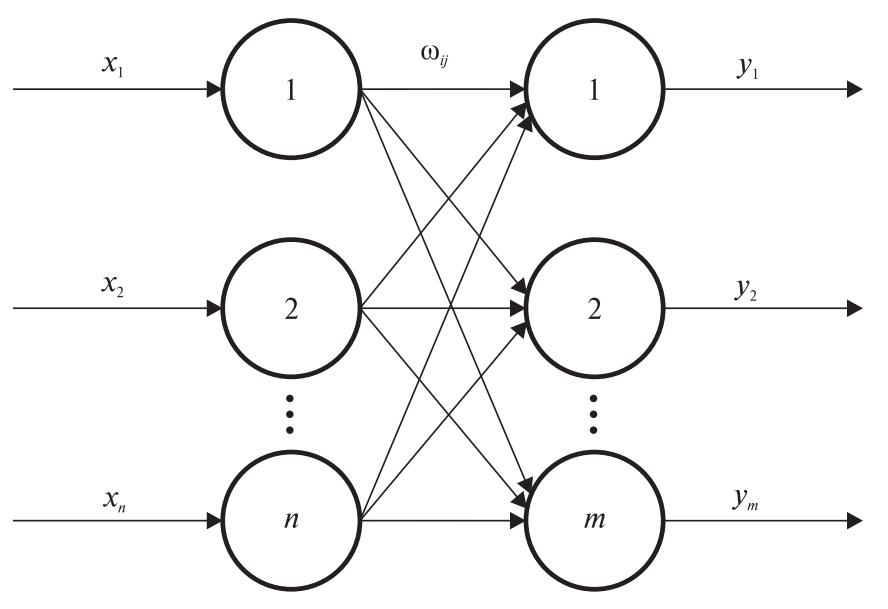
\includegraphics[scale=0.3]{author/part3/figures/neural_network.png}
	\caption{Пример архитектуры и.н.с.}
	\label{fig:nn_example}
\end{figure}

	Такая формулировка предполагает существование определенной нейросетевой архитектуры, которая определяет структурную конфигурацию модели.
	
	Рассмотрим архитектурные компоненты подробнее.

\begin{SCn}
	\scnheader{формальный нейрон}
	\scnidtf{искусственный нейрон}
	\scnidtf{нейрон}
	\scnidtf{ф.н.}
	\scnidtf{нейронный элемент}
	\scnidtf{множество нейронов искусственных нейронных сетей}
	\scnidtf{математическая модель биологического нейрона}
	\scnsubset{искусственная нейронная сеть}
	\scntext{пояснение}{Основной элемент \scnkeyword{и.н.с.}, применяющий свою \scnkeyword{функцию активации} [\scncite{Golovko2017}] к сумме произведений входных сигналов на весовые коэффициенты:
	\begin{equation*}
		y = F\left(\sum_{i=1}^{n} w_ix_i - T\right) = F(WX - T)
	\end{equation*}
	где $X = (x_1,x_2,...,x_n)^{T}$ -- вектор входного сигнала; $W - (w_1,w_2,...,w_n)$ -- вектор весовых коэффициентов; \textit{T} -- пороговое значение;
	\textit{F} -- \scnkeyword{функция активации}.}
\end{SCn}

Отдельный формальный нейрон является искусственной нейронной сетью с одним нейроном в единственном слое.

Пример описания одного нейрона в SCg представлен на рисунке \textit{\nameref{fig:nn_scg}}.

\begin{figure}[H]
	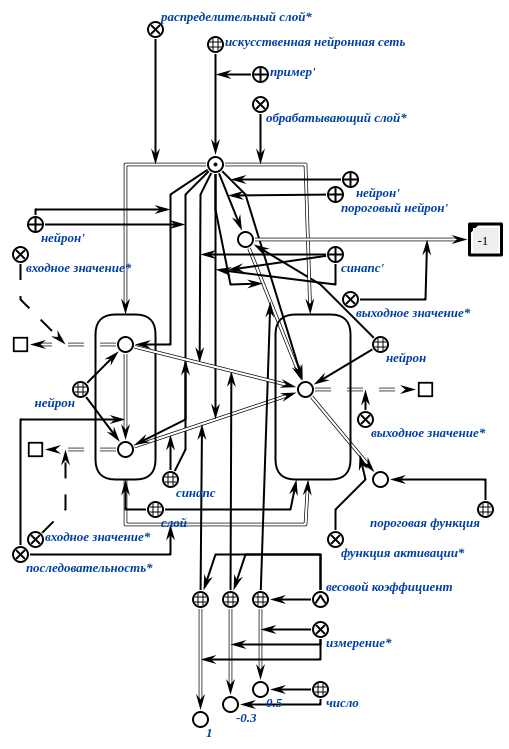
\includegraphics[scale=0.8]{author/part3/figures/neural_network_scg.png}
	\caption{Представление одного нейрона в SCg}
	\label{fig:nn_scg}
\end{figure}

Формальные нейроны могут быть классифицированы следующим образом:

\begin{itemize}
		\item полносвязный формальный нейрон -- нейрон, у которого есть полный набор связей с нейронами предшествующего слоя. Oтдельный обрабатывающий элемент \scnkeyword{и.н.с.}, выполняющий функциональное преобразование взвешенной суммы элементов вектора входных значений с помощью \scnkeyword{функции активации}
	 \item сверточный формальный нейрон -- отдельный обрабатывающий элемент \scnkeyword{и.н.с.}, выполняющий функциональное преобразование результата операции свертки матрицы входных значений с помощью \scnkeyword{функции активации}. Сверточный \scnkeyword{формальный нейрон} может быть представлен полносвязным \scnkeyword{формальным нейроном}.
	\item рекуррентный \scnkeyword{формальный нейрон} -- нейрон, имеющий обратную связь с самим собой или с другими нейронами \scnkeyword{и.н.с.}
\end{itemize}

Схематически формальный нейрон можно представить в виде следующей модели (рисунок \textit{\nameref{fig:formal_neuron}}).

\begin{figure}[H]
	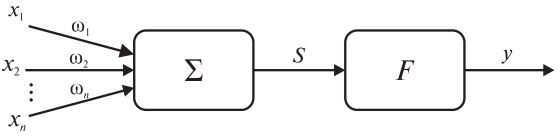
\includegraphics[scale=0.8]{author/part3/figures/formal_neuron.png}
	\caption{Формальный нейрон}
	\label{fig:formal_neuron}
\end{figure}

Определим понятие \scnkeyword{синаптическая связь} и \scnkeyword{слой и.н.с.}:

\begin{SCn}
	\scnheader{синаптическая связь}
	\scnidtf{синапс}
	\scnsubset{ориентированная пара}
	\scntext{пояснение}{ориентированная пара, первым компонентом которой является нейрон, из
	которого исходит сигнал, а вторым компонентом -- нейрон, который принимает этот сигнал}
\end{SCn}


\begin{SCn}
	\scnheader{слой и.н.с.}
	\scnidtf{слой}
	\scnidtf{слой искусственной нейронной сети}
	\scnidtf{множество слоев искусственных нейронных сетей}
	\scnsubset{искусственная нейронная сеть}
	\scntext{пояснение}{множество нейронных элементов, на которые в каждый такт времени
		параллельно поступает информация от других нейронных элементов сети [\scncite{Golovko2017}]}
	\scntext{пояснение}{множество формальных нейронов, осуществляющих параллельную независимую обработку вектора или матрицы входных значений}
\end{SCn}

Отдельный слой является искусственной нейронной сетью с одним слоем.

Следует отметить принципиальную важность этого замечания. Один \scnkeyword{слой и.н.с.}  уже является нейронной сетью, поскольку над ним можно производить все основные операции, которые производятся над ``большой'' \scnkeyword{и.н.с.} (его можно обучить и использовать для решения определенной задачи).

\scnkeyword{Слои и.н.с.} могут быть классифицированы следующим образом (по признаку операции, осуществляемой слоем):
\begin{itemize}
		\item полносвязный слой и.н.с. -- слой, в котором каждый нейрон является полносвязным
		\item сверточный слой и.н.с. -- слой, в котором каждый нейрон является сверточным
		\item слой и.н.с. нелинейного преобразования -- слой, осуществляющий нелинейное преобразование входных данных
		\item dropout слой и.н.с. -- слой, реализующий технику регуляризации dropout
		\item pooling слой и.н.с. -- подвыборочный слой
		\item слой и.н.с. батч-нормализации
\end{itemize}

Как правило, слой нелинейного преобразования  выделяется в отдельный слой только в программных реализациях. Фактически он рассматривается как финальный этап расчета выходной активности любого нейрона -- применение \scnkeyword{функции активации}.

Dropout-слой функционирует только во время обучения \scnkeyword{и.н.с.} Поскольку полносвязные слои имеют большое количество настраиваемых параметров, они подвержены эффекту \scnkeyword{переобучения}. Один из способов устранить такой негативный эффект -- выполнить частичный отсев результатов на выходе полносвязного слоя. На этапе обучения техника dropout позволяет отбросить выходную активность некоторых нейронов с определенной, заданной вероятностью. Выходная активность ``отброшенных'' нейронов полагается равной нулю.

Назначение подвыборочного слоя -- в осуществлении уменьшения размерности входных данных.

Нужно отметить, что данный перечень неполный -- разновидности \scnkeyword{слоев и.н.с.} появляются практически в каждой заслуживающей внимания публикации по нейросетевым алгоритмам и на текущий момент их существует достаточно много, однако, как правило, при построении более традиционных архитектур ограничиваются только приведенными вариантами слоев.

\scnkeyword{Слои и.н.с.} также могут быть классифицированы по исполняемой роли в рамках архитектуры (место в последовательности \scnkeyword{слоев и.н.с.}).

Так, например, слой, расположенный первым, называется распределяющим. Слои, расположенные далее, за исключением последнего, называются обрабатывающими. Наконец, последний слой носит название выходного \scnkeyword{слоя и.н.с.}

Наконец, последний архитектурный компонент \scnkeyword{и.н.с.} -- это функция активации:

\begin{SCn}
	\scnheader{функция активации*}
	\scnidtf{функция активации нейрона*}
	\scniselement{неролевое отношение}
	\scniselement{бинарное отношение}
	\scntext{пояснение}{неролевое отношение, связывающее формальный нейрон с функцией, результат
		применения которой к \textbf{\textit{взвешенной сумме нейрона}} определяет его \textbf{\textit{выходное значение}}.}
	%\scnrelfrom{область определения}{
		
	%}
    %\scnreltoset{объединение}{формальный нейрон;функция}
	\scnrelfrom{первый домен}{формальный нейрон}
	\scnrelfrom{второй домен}{функция}
\end{SCn}

Перечислим некоторые, наиболее известные и применяемые типы функций активации:
\begin{itemize}
	\item линейная функция\\
	\scntext{формула}{
		\begin{equation*}
			y = kS
		\end{equation*}
		где \textit{k} -- коэффициент наклона прямой, \textit{S} -- в.с.
	}
	\item пороговая функция\\
	\scntext{формула}{
		\begin{equation*}
			y = sign(S) =
			\begin{cases}
				1, S > 0,\\
				0, S \leq 0
			\end{cases}
		\end{equation*}
	}
	\item сигмоидная функция\\
	\scntext{формула}{
		\begin{equation*}
			y = \frac{1}{1+e^{-cS}}
		\end{equation*}
		где \textit{с} > 0 -- коэффициент, характеризующий ширину сигмоидной функции по оси абсцисс, \textit{S} -- в.с.
	}
	\item функция гиперболического тангенса\\
	\scntext{формула}{
		\begin{equation*}
			y = \frac{e^{cS}-e^{-cS}}{e^{cs}+e^{-cS}}
		\end{equation*}
		где \textit{с} > 0 -- коэффициент, характеризующий ширину сигмоидной функции по оси абсцисс, \textit{S} -- в.с.
	}
	\item функция softmax\\
	\scntext{формула}{
		\begin{equation*}
			y_j = softmax(S_j) = \frac{e^{S_j}}{\sum_{j} e^{S_j}}
		\end{equation*}
		где $S_j$ -- в.с. \textit{j}-го выходного нейрона
	}
	\item функция ReLU\\
	\scntext{формула}{
		\begin{equation*}
			y = F(S) =
			\begin{cases}
				S, S > 0,\\
				kS, S \leq 0
			\end{cases}
		\end{equation*}
		где \textit{k} = 0 или принимает небольшое значение, например, 0.01 или 0.001.
	}
\end{itemize}

\subsection{Денотационная семантика моделей искусственных нейронных сетей, используемых в ostis-системах}

\subsection{Операционная семантика моделей искусственных нейронных сетей, используемых в ostis-системах}

Рассмотрим основные действия, выполняемые с \scnkeyword{и.н.с.}

\begin{itemize}
	\item действие конфигурации и.н.с.
	\begin{itemize}
		\item действие создания и.н.с.
		\item действие редактирования и.н.с.
		\item действие удаления и.н.с.
		\item действие конфигурации слоя и.н.с.
		\begin{itemize}
			\item действие добавления слоя в и.н.с.
			\item действие редактирования слоя и.н.с.
			\item действие удаления слоя и.н.с.
			\item действие установки функции активации нейронов слоя и.н.с.
			\item действие конфигурации нейрона в слое и.н.с.
			\begin{itemize}
				\item действие добавления нейрона в слой и.н.с.
				\item действие редактирования нейрона в слое и.н.с.
				\item действие удаления нейрона из слоя и.н.с.
				\item действие установки функции активации нейрона в слое и.н.с.
			\end{itemize}
		\end{itemize}
	\end{itemize}
	\item действие конфигурации настраиваемых параметров и.н.с.
	\item действие интерпретации и.н.с.
\end{itemize}

Первый тип разновидностей действий относится к архитектурному изменению \scnkeyword{и.н.с.}, который влияет на ее структуру. Второй тип связан с начальной инициализацией настраиваемых параметров нейронной сети и ее обучением. Наконец третий тип действий связан с интерпретированием результатов, получаемых нейронной сетью и, в целом, может рассматриваться как действие по использованию (применению) \scnkeyword{и.н.с.} для решения конкретной задачи.

Действия по обработке \scnkeyword{и.н.с.} осуществляет соответствующий коллектив агентов. 

Так как в результате действий по обработке и.н.с. объект этих действий, конкретная и.н.с., может существенно меняться (меняется конфигурация сети, ее весовые коэффициенты), то и.н.с. представляется в базе знаний как темпоральное объединение всех ее версий. Каждая версия является  \scnkeyword{и.н.с.} и темпоральной сущностью. На множестве этих темпоральных сущностей задается темпоральная последовательность с указанием первой и последней версии. Для каждой версии описываются специфичные знания.

Общие для всех версий знания описываются для и.н.с, являющейся темпоральным объединением всех версий (рисунок \textit{\nameref{fig:temporal_neural_network_scg}})

\begin{figure}[H]
	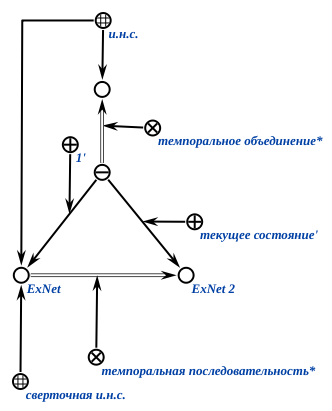
\includegraphics[scale=0.8]{author/part3/figures/temporal_neural_network_scg.png}
	\caption{Темпоральность нейронной сети}
	\label{fig:temporal_neural_network_scg}
\end{figure}

Далее более подробно рассмотрим действие по обучению \scnkeyword{и.н.с.} и сделаем обзор основных методов, применяемых для обучения.

Действие обучения  \scnkeyword{и.н.с.} -- действие, в ходе которого реализуется определенный метод обучения  \scnkeyword{и.н.с.} с заданными параметрами обучения  \scnkeyword{и.н.с.}, методом оптимизации и функцией потерь.

При обучении возможно возникновение следующих проблем:

\begin{itemize}
	\item Переобучение -- проблема, возникающая при обучении  \scnkeyword{и.н.с.}, заключающаяся в том,
	что сеть хорошо адаптируется к паттернам входной активности из обучающей выборки, при этом теряя способность к обобщению.
	Переобучение возникает из-за применения неоправданно сложной модели при обучении  \scnkeyword{и.н.с.} Это происходит,
	когда количество настраиваемых параметров и.н.с. намного больше размера обучающей выборки. Возможные
	варианты решения проблемы заключаются в упрощении модели, увеличении выборки, использовании регуляризации
	(параметр регуляризации, техника dropout и т.д.).\\
	Обнаружение переобученности сложнее, чем недообученности. Как правило, для этого применяется
	кросс-валидация на валидационной выборке, позволяющая оценить момент завершения процесса обучения.
	Идеальным вариантом является достижение баланса между переобученностью и недообученностью.
	
	\item Недообучение -- проблема, возникающая при обучении  \scnkeyword{и.н.с.}, заключающаяся в том,
	что сеть дает одинаково плохие результаты на обучающей и контрольной выборках.
	Чаще всего такого рода проблема возникает при недостаточном времени, затраченном на обучение модели.
	Однако это может быть вызвано и слишком простой архитектурой модели либо малым размером обучающей
	выборки. Соответственно решение, которое может быть принято ML-инженером, заключается в устранении
	этих недостатков: увеличение времени обучения, использование модели с большим числом настраиваемых
	параметров, увеличение размера обучающей выборки, а также уменьшение регуляризации и более тщательный
	отбор признаков для обучающих примеров.
\end{itemize}

Методом обучения \scnkeyword{и.н.с.} называется процесс итеративного поиска оптимальных значений настраиваемых параметров и.н.с., минимизирующих некоторую заданную функцию потерь.

Стоит отметить, что хотя целью применения метода обучения является минимизация функции потерь, ``полезность'' полученной после обучения модели можно оценить только по достигнутому уровню ее обобщающей способности.

Методы обучения могут быть поделены на две большие группы -- \textit{\textbf{методы обучения с учителем}} и \textit{\textbf{методы обучения без учителя}} (контролируемый и неконтролируемый методы обучения).

Метод обучения с учителем -- метод обучения с использованием заданных целевых переменных.

Одним из методов обучения с учителем является метод обратного распространения ошибки.

Приведем его описание в виде алгоритма:

\begin{algorithm}[H]
	\KwData{$X$ -- данные, $E_t$ -- желаемый отклик (метки), $E_m$ -- желаемая ошибка (в соответствии с выбранной функцией потерь)}
	\KwResult{обученная нейронная сеть \textit{Net}}
	инициализация весов \textit{W} и порогов \textit{T};\\
	\Repeat{$E<E_m$}{
		\ForEach{$x \in X$, $e \in E_t$}{
			фаза прямого распространения сигнала: вычисляются активации для всех слоев и.н.с.;\\
			фаза обратного распространения ошибки: вычисляются ошибки для последнего слоя и всех предшествующих слоев;\\
			изменение настраиваемых параметров и.н.с. в соответствии с вычисленными ошибками;\\
		}
		вычисление общей ошибки E на данной эпохе;
	}
\end{algorithm}

Метод обратного распространения ошибки использует заданный метод оптимизации и заданную функцию потерь для реализации фазы обратного распространения ошибки и изменения настраиваемых параметров и.н.с. Одним из самых распространенных методов оптимизации является метод стохастического градиентного спуска. Приведенный метод используется для реализации последовательного варианта обучения.

Следует также отметить, что несмотря на то, что метод отнесен к методам обучения с учителем, в случае
его использования для обучения автокодировщиков в классических публикациях он рассматривается как
метод обучения без учителя, поскольку в данном случае размеченные данные отсутствуют.

\textbf{\textit{Метод обучения без учителя}} -- метод обучения без использования заданных целевых переменных (в режиме самоорганизации)

В ходе выполнения алгоритма метода обучения без учителя выявляются полезные структурные свойства
набора. Неформально его понимают как метод для извлечения информации из распределения, выборка для которого
не была вручную аннотирована человеком [\scncite{Goodfellow2017}]. Метод обучения без учителя может рассматриваться как вспомогательный метод для начальной инициализации настраиваемых параметров и.н.с. В этом случае он является методом предобучения.

Среди методов, применяемых для оптимизации целевой функции можно выделить следующие:

\begin{itemize}
	\item SGD (стохастический градиентный спуск): в данном методе корректировка настраиваемых параметров и.н.с. выполняется в направлении максимального уменьшения функции стоимости, т.е. в направлении, противоположном вектору градиента функции потерь [\scncite{Haykin2006}]
	\item метод Нестерова: Обучение методом стохастического градиентного спуска иногда происходит очень медленно. Импульсный метод позволяет ускорить обучение, особенно в условиях высокой кривизны, небольших, но устойчивых градиентов или зашумленных градиентов. В импульсном методе вычисляется экспоненциально затухающее скользящее среднее прошлых градиентов и продолжается движение в этом направлении. Метод Нестерова является вариантом импульсного алгоритма, в котором градиент вычисляется после применения текущей скорости [\scncite{Goodfellow2017}]
	\item AdaGrad: Данный метод по отдельности адаптирует скорости обучения всех настраиваемых параметров и.н.с., умножая их на коэффициент, обратно пропорциональный квадратному корню из суммы всех прошлых значений квадрата градиента [\scncite{Duchi2011}]
	\item RMSProp: Данный метод является модификацией AdaGrad, которая позволяет улучшить его поведение в невыпуклом случае путем изменения способа агрегирования градиента на экспоненциально взвешенное скользящее среднее. Использование экспоненциально взвешенного скользящего среднего гарантирует повышение скорости сходимости после обнаружения выпуклой впадины, как если бы внутри этой впадины алгоритм AdaGrad был инициализирован заново [\scncite{Goodfellow2017}]
	\item Adam: Данный метод можно рассматривать как комбинацию RMSProp и AdaGrad [\scncite{Kingma2014}]. Помимо усредненного первого момента, данный метод использует усредненное значение вторых моментов градиентов
\end{itemize} 

Отметим, что успешность применения методов оптимизации зависит главным образом от знакомства пользователя с соответствующим алгоритмом [\scncite{Goodfellow2017}].

Еще одним важным компонентом, влияющим на процесс обучения, является используемая функция потерь.

\scnkeyword{Функция потерь} -- функция, используемая для вычисления ошибки, рассчитываемой как разница между фактическим эталонным значением и прогнозируемым значением, получаемым \scnkeyword{и.н.с.}

Среди функций потерь, используемые в качестве целевых функций для применяемого метода оптимизации, можно выделить:

\begin{itemize}
	\item MSE -- средняя квадратичная ошибка\\
		\begin{equation*}
			MSE = \frac{1}{L} \sum_{l=1}^L \sum_{i=1}^m (y_i^l - e_i^l)^2
		\end{equation*}
		где $y_i^l$ -- прогноз модели, $e_i^l$ -- ожидаемый (эталонный) результат, \textit{m} -- размерность выходного вектора, \textit{L} -- объем обучающей выборки.

	\item BCE -- бинарная кросс-энтропия\\
	\begin{equation*}
		BCE = - \sum_{l=1}^L (e^l \log(y^l) + (1 - e^l)\log(1 - y^l))
	\end{equation*}
	где $y^l$ -- прогноз модели, $e^l$ -- ожидаемый (эталонный) результат: \textit{0} или \textit{1}, \textit{L} -- объем обучающей выборки.
	\item MCE -- мультиклассовая кросс-энтропия\\
	\begin{equation*}
		MCE = - \sum_{l=1}^L \sum_{i=1}^m e_{i}^l \log(y_{i}^l)
	\end{equation*}
	где $y_{i}^l$ -- прогноз модели, $e_i^l$ -- ожидаемый (эталонный результат), \textit{m} -- размерность выходного вектора
\end{itemize}

Отметим, что для бинарной кросс-энтропии в выходном слое \scnkeyword{и.н.с.} будет находиться один нейрон, а для для мультиклассовой кросс-энтропии количество нейронов в выходном \scnkeyword{слое и.н.с.} совпадает с количеством классов.

Для решения задачи классификации рекомендуется использовать бинарную или мультиклассовую кросс-энтропийную функцию потерь, для решения задачи регрессии рекомендуется использовать среднюю квадратичную ошибку.

Действие обучения \scnkeyword{и.н.с.} можно проиллюстрировать следующим изображением \textit{\nameref{fig:ann_training_nn_scg}}.

\begin{figure}[H]
	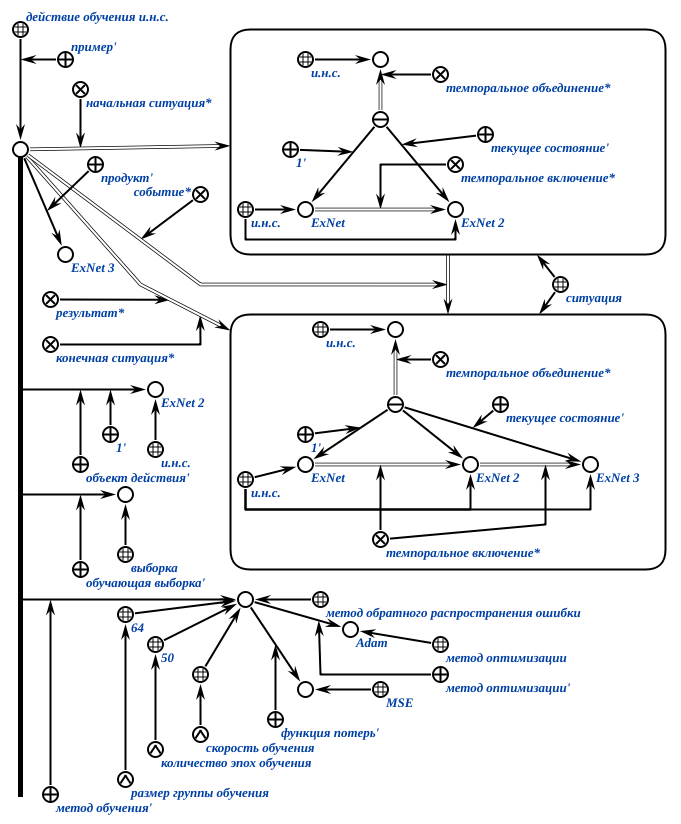
\includegraphics[scale=0.8]{author/part3/figures/ann_training_nn_scg.png}
	\caption{Действие обучения и.н.с.}
	\label{fig:ann_training_nn_scg}
\end{figure}

\section{Логико-семантическая модель ostis-системы автоматизации проектирования искусственных нейронных сетей, семантически совместимых с базами знаний ostis-систем}

Наличия языка представления нейросетевых методов на SCP и его интерпретатора позволяет обеспечить интерпретацию нейросетевого метода в памяти ostis-системы. Наличие в единой памяти не только экземпляров методов, но и понятий, их описывающих, создает основу для автоматизации процесса построения нейросетевых методов. В памяти ostis-системы хранятся знания о том, методы какого класса могут решить задачу заданного класса, но экземпляров класса этого метода может не быть представлено в системе. На этот случай система должна иметь возможность сообщить пользователю о возможности решения, для которого, однако, необходимо погрузить в систему определенный метод. Так как система хранит в единой памяти задачу и требования к методу ее решения, появляется возможность спроектировать необходимый метод. Для этого необходимо наличие среды проектирования методов соответствующих классов. В случае нейросетевого метода, речь идет об интеллектуальной среде построения нейросетевых методов.

В основе интеллектуальной среды построения нейросетевых методов лежат соответствующие другу другу иерархии действий, задач и методов построения и.н.с. Наличие такой иерархии позволит описать язык представления методов построения и.н.с. и разработать интерпретатор этого языка.

Построение иерархии соответствующих действий построения и.н.с. следует начать с изучения этапов проектирования и обучения и.н.с., которые, в общем случае, выполняют все разработчики и.н.с.:

\textbf{1. Постановка задачи. }

Постановка задачи включает в себя описание входных данных (изображения/видео, временные ряды, текст), выходных данных и требований к методу решения (скорость, затраты по памяти и т.д.). Также описывается дополнительная информация, которая может помочь в построении метода решения задачи (к примеру, спецификация обучающей выборки, если таковая имеется). Обычно, на данном этапе разработчик и.н.с. определяет класс задачи, формирует требования к обучающей выборке, если она не предоставлена.

Выполнение данного этапа средой проектирования и.н.с. подразумевает выполнение следующих действий:
\begin{itemize}
	\item \textit{Действие трансляции условия задачи}. Действие транслирует заданное с помощью интерфейса ostis-системы (к примеру, естественно-языкового интерфейса) описание задачи в память ostis-системы.  Действие необходимо в случае, когда условие задачи задается пользователем. Необходимо понимать, что описание задачи поступает в базу знаний не только от пользовательского интерфейса. К примеру, задача может быть сформулирована самой системой в ходе ее жизнедеятельности.
	Данное действие является общим для всех ostis-систем, поэтому его рассмотрение выходит за рамки рассмотрения процесса построения интеллектуальной среды проектирования и.н.с.
	\item \textit{Действие классификации задачи}. Действие определяет класс задачи (задача регрессии, детекции, кластеризации и т.д.), исходя из описания задачи в базе знаний.
	\item \textit{Действие поиска подходящей обучающей выборки}. В базе знаний может храниться набор спецификаций выборок, к которым у ostis-системы есть доступ. Действие производит поиск выборок, которые могут быть использованы в качестве обучающей выборки.
	\item \textit{Действие формирования требования к обучающей выборки}. Если обучающая выборка не была предоставлена и не была найдена, то необходимо сформировать описание требований к обучающей выборке, которое можно будет транслировать на язык пользовательского интерфейса и затребовать необходимую выборку у пользователя.
\end{itemize}

\textbf{2. Предобработка выборки: очистка}

На этом этапе обнаруживаются признаки, которые имеют в общем случае некорректные значения (например, для каких-то образов значение признака может иметь неопределенное значение, либо значение, не совпадающее по типу, либо аномально большое или очень маленькое значение, которое встречается в редком числе случаев).  Для признаков, имеющих неопределенное значение, может быть применены различные методы устранения, например, такие значения могут быть заменены средним значением этого признака, рассчитанным по всем образам (для непоследовательных данных), либо они могут быть заменены средним значениям по соседним образам (в случае временных рядов), либо каким-то фиксированным значением. Радикальная мера решения проблемы -- удаление образов, имеющих неопределенные значения признаков из выборки. Однако его лучше применять, если образов с отсутствующими значениями признаков немного. Для выбросов и аномалий применяются схожие стратегии (но только в том случае, если задача не состоит в прогнозировании этих аномалий).

В интеллектуальной среде проектирования данный этап соответствует выполнению \textit{действия очистки выборки}, которое выполняется в случае обработки выборки, которая ранее не была представлена в памяти системы (к примеру, была получена от пользователя). 
Реализация интерпретатора (агента) данного действия требует описания в памяти классификации стратегий очистки данных и реализации методов применения этих стратегий. 

\textbf{3. Предобработка выборки: выявление содержательных признаков}

Осуществляется т.н. инжиниринг признаков, состоящий в отборе признаков, влияющих на результат работы модели, несодержательные признаки, которые никак не коррелируют с выходом модели, удаляются. Цель этого этапа -- уменьшение размерности пространства признаков для снижения влияния эффекта переобучения на модель.

Для снижения размерности признакового пространства может применяться методы отбора признаков и выделения признаков.

При отборе признаков, осуществляется формирование подмножества из исходных признаков (алгоритм последовательного обратного отбора, рекурсивный алгоритм обратного устранения признаков,  алгоритмы с использованием случайных лесов). 

При выделении признаков из набора признаков извлекается информация для построения нового подпространства признаков (алгоритмы с использованием автоэнкодера).

В интеллектуальной среде проектирования данный этап соответствует выполнению \textit{действия выявления содержательных признаков}. Реализация интерпретатора(агента) данного действия требует описания в памяти классификации стратегий снижения размерности признакового пространства и реализации методов применения этих стратегий. 

\textbf{4. Предобработка выборки: трансформация}

На этом этапе осуществляется подготовка данных к обучению. 
Здесь следует уделить особое внимание наличию категориальных признаков, чаще всего заданных строковыми типами. Эти признаки могут быть номинальными и порядковыми. Для кодирования порядковых признаков чаще всего применяют последовательный числовой код (1, 2, 3,...). Для кодирования номинальных такое решение неверно, т.к. эти признаки равноправны и не могут сравниваться по числовому коду (например, пол -- 0/1). Для номинальных признаков применяется способ прямого кодирования, заключающийся в создании и использовании фиктивных признаков по количеству значений исходного. Например, признак пол (мужской, женский) преобразуется в два новых признака мужской и женский с соответствующими значениями для имеющихся образов.

Масштабирование признаков предполагает приведение значений признаков к одному общему интервалу -- это особенно актуально для признаков, имеющих несоразмерные выборочные средние значения по всем образам -- например, один признак в среднем имеет значение 10.000, а другой 12. Это может проявится в выполнении минимизации только по признаку с наибольшими значениями и плохой сходимости метода обучения. Чаще всего масштабирование соответствует выполнению нормализации на отрезок (min-max нормализация):

\begin{equation*}
	x_{norm}^i = \frac{x^i - x_{min}}{x_{max} - x_{min}}
\end{equation*}
где $x^i$ -- значение признака   для отдельно взятого образа \textit{i}, $x_{min}$ -- наименьшее значение для признака, $x_{max}$ -- наибольшее значение для признака.

Другой вариант масштабирования -- применение стандартизации признаков:

\begin{equation*}
	x_{std}^i = \frac{x^i - \mu(x)}{\sigma(x)},
\end{equation*}
$\mu(x)$ -- выборочное среднее отдельного признака, $\sigma(x)$ -- стандартное отклонение.

Стандартизация сохраняет полезную информацию о выбросах в исходных данных и делает алгоритм обучения менее чувствительным к ним.

Дискретизация применяется для перехода от вещественного признака к порядковому за счет кодирования интервалов одним значением (например, если признак отражает возраст человека, то может быть произведена дискретизация значений с выделением определенных возрастных групп, где каждая группа будет кодироваться одним целым числом).

В интеллектуальной среде проектирования данный этап соответствует выполнению \textit{действия трансформации выборки}. Реализация интерпретатора(агента) данного действия требует описания в памяти классификации методов масштабирования признаков и реализации методов применения этих стратегий. 

\textbf{5. Разбиение выборки на обучающую, валидационную и тестовую (контрольную)}

Производится разбиение всей выборки данных, на обучающую, тестовую и, в некоторых случаях, валидационную.

Валидационная выборка используется для оценки влияния изменения гиперпараметров на результат обучения и может применяться как дополнительный инструмент для этого наравне с сеточным поиском.

Разбиение проводится в соотношении 3:1:1, в процентах (60/20/20), если валидационная выборка не используется, то 80/20.

В интеллектуальной среде проектирования данный этап соответствует выполнению \textit{действия разбиения выборки}.

Все предыдущие этапы применялись к выборке, последующие этапы относятся к используемым моделям и.н.с.

\textbf{6. Выбор класса нейросетевых методов в соответствии со сформулированной задачей}

На этом этапе осуществляется выбор основной архитектуры и.н.с., которая будет использоваться при обучении. Однако, нужно отметить, что этот выбор относительно условный, т.е. исследователь не ограничен использованием только одного типа и.н.с. для решения задачи (как, например, сверточной сети для изображений, поскольку изображения можно обрабатывать и обычным многослойным персептроном). Речь скорее идет именно о рекомендованной архитектуре, но это не исключает использование любых других вариантов архитектур и их сочетаний в рамках одной модели).  

Примерами таких рекомендаций являются:
\begin{itemize}
	\item Изображения/видео -- сверхточные нейронные сети
	\item Временные ряды -- многослойные персептроны или рекуррентные сети
	\item Текстовая информация -- многослойные персептроны или рекуррентные сети
	\item Наборы характеристик некоторых объектов (например, спецификации автомобилей) -- многослойный персептрон
\end{itemize}

В интеллектуальной среде проектирования данный этап соответствует выполнению \textit{действия выбора класса нейросетевых методов}.

\textbf{7. Формирование спецификации на входные и выходные данные}

Выполняются дополнительные преобразования данных, связанные с изменением структур хранения (например, преобразование многомерного массива в одномерный, конвертация типов)

В интеллектуальной среде проектирования данный этап соответствует выполнению \textit{действия формирования спецификации входов и выходов и.н.с.}.

\textbf{8. Выбор метода оптимизации }

В рамках работы \cite{Kovalev2022} в рамках ПрО и.н.с. описаны следующие методы оптимизации:
\begin{itemize}
	\item стохастический градиентный спуск (SGD);
	\item метод Нестерова;
	\item адаптивный градиент(AdaGrad);
	\item адаптивная оценка момента (Adam);
	\item среднеквадратическое распространение (RMSProp).
\end{itemize}

В интеллектуальной среде проектирования данный этап соответствует выполнению \textit{действия выбора методо оптимизации}.

\textbf{9. Выбор минимизируемой функции ошибки}

На этом этапе задается функция ошибок, которая будет минимизироваться. К примеру, MSE лучше подходит для задач регрессии и для кластеризации, CE -- для классификационных задач.
В работе \cite{Kovalev2022} описана классификация таких функций в рамках ПрО и.н.с.

Данные функции определяются следующим образом:
\begin{equation*}
	MSE = \frac{1}{n} \sum_{i=1}^n (Y_i - \widetilde{Y_i})^2    
\end{equation*}
где \textit{n} -- размер обучающей выборки, $Y_i$ -- эталонное значение функции, $\widetilde{Y_i}$ -- результат, полученный НС

\begin{equation*}
	CE = - \frac{1}{n} \sum_{i=1}^n (Y_i\log(\widetilde{Y_i}) + (1-Y_i)\log(1 - \widetilde{Y_i}))    
\end{equation*}
(случай 2-классовой классификации)

\begin{equation*}
	CE = - \frac{1}{n} \sum_{i=1}^n \sum_{c=1}^M Y_i^c \log{\widetilde{Y}_i^c} 
\end{equation*}
(случай многоклассовой классификации)

В интеллектуальной среде проектирования данный этап соответствует выполнению \textit{действия выбора минимизируемой функции ошибки}.

\textbf{10. Начальная инициализация параметров нейронной сети}

В работе \cite{Kovalev2022} в рамках ПрО и.н.с. уже описаны методы начальной инициализации и.н.с. Наиболее часто используемые варианты инициализации весовых коэффициентов и порогов нейронной сети включают:
\begin{itemize}
	\item инициализация значениями из равномерного распределения на каком-то небольшом интервале, например, [-0.1, 0.1].
	\item инициализация значениями из стандартного нормального распределения.
	\item инициализация по методу Ксавье \cite{glorot2010}.
	
	Применяется для предотвращения  резкого уменьшения или увеличения значений выхода нейронных элементов после применения функции активации при прямом прохождении образа через глубокую нейронную сеть. Фактически инициализация этим методом осуществляется посредством выбора значений из равномерного распределения на отрезке $[- \sqrt{6} / \sqrt{n_i+n_{i+1}}, \sqrt{6} / \sqrt{n_i+n_{i+1}}]$, где $n_i$ -- это число входящих связей в данный слой, а $n_i$ -- число исходящих связей из данного слоя. Таким образом, инициализация этим методом проводится для разных слоев нейронной сети из разных отрезков.
	
	\item инициализация, полученная из предобученной модели.
	
	Вариант инициализации, который предполагает использование в качестве ``стартовой'' модели предобученной модели, взятой из некоторого репозитория предобученных моделей, обученную самим исследователем или в процессе работы интеллектуальной системы.
	
	\item инициализация по методу Кайминга \cite{he2015}.
	
	Данный метод инициализации применяется для решения проблемы ``затухающего'' градиента и ``взрывающегося''
	градиента. Производится посредством выбора значений из равномерного распределения на отрезке $[-\sqrt{2} / \sqrt{(1+a^2)fan}, \sqrt{2} / \sqrt{(1+a^2)fan}]$,
	где \textit{a} -- угол наклона к оси абсцисс для отрицательной части области определения функции активации типа ReLU (для обычной ReLU функции этот параметр равен 0), $fan$ -- параметр режима работы, который для фазы прямого распространения равен количеству входящих связей (для устранения эффекта ``взрывающегося'' градиента), а для фазы обратного распространения -- количеству выходящих (для устранения эффекта ``затухающего'' градиента).
\end{itemize}

В интеллектуальной средепроектирования данный этап соответствует выполнению \textit{действия начальной инициализации и.н.с.}.

\textbf{11. Выбора гиперпараметров и.н.с.}

На практике некоторые гиперпараметры (такие как количество слоев, их типы, количество нейронов в слое) часто определяются экспериментально, в процессе итеративного поиска лучшего варианта решения задачи. Хотя способы частично автоматизировать этот процесс существуют, они все же рассчитаны на наличие некоторых предусловий проведения эксперимента, в частности интервалов изменения параметра (например, скорости обучения).

К гиперпараметрам, подбираемым на этом этапе, относятся:
\begin{itemize}
	\item Параметры обучения и.н.с. (скорость обучения, моментный параметр, размер мини-батча).
	\item Архитектура модели и.н.с., опирающаяся на ранее сформулированные спецификации входных и выходных данных (например, количество нейронов в определенном слое (слоях) или конфигурации целых слоев)
\end{itemize}

Нахождение оптимальных гиперпараметров может быть получено, например, использованием метода сеточного поиска, который позволяет проверить значения гиперпараметров, взятые с определенным шагом или из определенного интервала (кортежа). С помощью этого метода выбирается оптимальный набор гиперпараметров, который дает лучшие результаты, он используется для последующего дообучения. Или же, если полученные результаты являются приемлемыми, то процесс дальнейшего обучения вообще не проводится. Следует отметить затратность данного метода, т.к. фактически осуществляется перебор различных значений параметров обучения. Для снижения объема работы применяется метод случайного поиска.

Для оптимизации архитектуры определяются типы слоев нейронной сети, количество нейронных элементов в каждом слое, их характеристики -- функция активации, для сверточных элементов -- размер ядра, а также  параметры padding и шаг свертки (stride).
Здесь же может осуществляться оценка не только пользовательского варианта сети, но и предобученной архитектуры. Основное правило при выборе -- количество параметров модели не должно превышать размер обучающей выборки. Для предобученных архитектур это ограничение снимается.

В интеллектуальной среде проектирования данный этап соответствует выполнению \textit{действия выбора гипперпараметров и.н.с.}. Действие использует классификацию и спецификации гиперпараметров и.н.с. (описаны в рамках ПрО и.н.с. \cite{Kovalev2022}). 

\textbf{12. Обучение модели на обучающей выборке}

Производится обучение модели до достижения выбранной точности (оценивается на тестовой выборке) или по другим заданным критериям (достижение заданного количества эпох обучения, неизменность точности на протяжении заданного количества эпох, падение точности на валидационной выборке и т.д.)

Алгоритмы обучения уже описаны в ПрО и.н.с.\cite{Kovalev2022}. Здесь приведем их классификацию:
\begin{SCn}
	\scnheader{метод обучения и.н.с.}
	\scnsubset{метод}
	\scnsuperset{метод обучения с учителем}
	\begin{scnindent}
		\scntext{explanation}{
			\textbf{\textit{метод обучения с учителем}} -- метод обучения с использованием заданных целевых переменных.
		}
		\scnsuperset{метод обратного распространения ошибки}
		\begin{scnindent}
			\scnidtf{м.о.р.о.}
			\scntext{explanation}{м.о.р.о. использует заданный метод оптимизации и заданную функцию потерь для реализации фазы обратного распространения ошибки и изменения настраиваемых параметров и.н.с. Одним из самых распространенных
				методов оптимизации является метод стохастического градиентного спуска. 
				}
				\scntext{explanation}{Следует также отметить, что несмотря на то, что метод отнесен к методам обучения с учителем, в случае
					использования м.о.р.о. для обучения автокодировщиков в классических публикациях он рассматривается как
					метод обучения без учителя, поскольку в данном случае размеченные данные отсутствуют.
					}
				\end{scnindent}
			\end{scnindent}
			\scnsuperset{метод обучения без учителя}
			\begin{scnindent}
				\scntext{explanation}{\textbf{\textit{метод обучения без учителя}} -- метод обучения без использования заданных целевых переменных(в режиме самоорганизации)
					}
					\scntext{explanation}{В ходе выполнения алгоритма метода обучения без учителя выявляются полезные структурные свойства
						набора. Неформально его понимают как метод для извлечения информации из распределения, выборка для которого
						не была вручную аннотирована человеком \cite{Goodfellow2017}.
						}
					\end{scnindent}
				\end{SCn}
				
				В интеллектуальной среде проектирования данный этап соответствует выполнению \textit{действия обучения и.н.с.}. Пример формализации данного действия представлен на рисунке \ref{fig:ann_trainning_scg}
				
				\begin{figure}
					\centering
					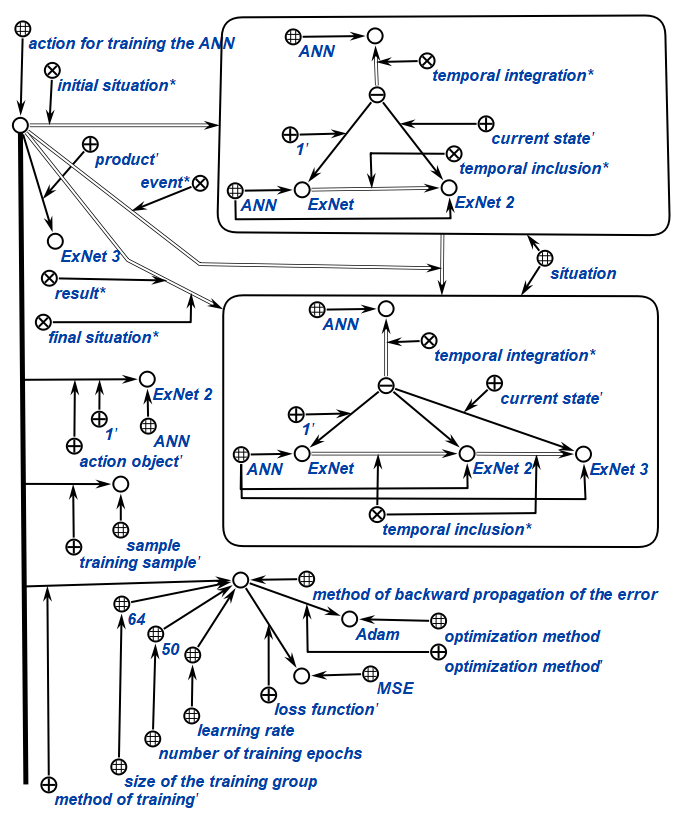
\includegraphics[width=0.9\linewidth]{author/part3/figures/ann_trainning_en.png}
					\caption{Пример формализации действия обучения искусственной нейронной сети в базе знаний \cite{Kovalev2022}}
					\label{fig:ann_trainning_scg}
				\end{figure}
				
				\textbf{13. Оценка эффективности и.н.с}
				
				После выполнения обучения осуществляется оценка полученной модели с помощью метрик оценки качества.
				
				Далее результат оценки может быть визуализирован с помощью матрицы ошибок (confusion matrix) и ROC-кривой.
				
				Матрица ошибок представляется собой матрицу (рис. \ref{fig:conf_matrix}), в которую помещены сведения о числе истинно-положительных, истинно-отрицательных, ложно-положительных и ложно-отрицательных предсказаниях классификатора.
				
				\begin{figure}[h]
					\centering
					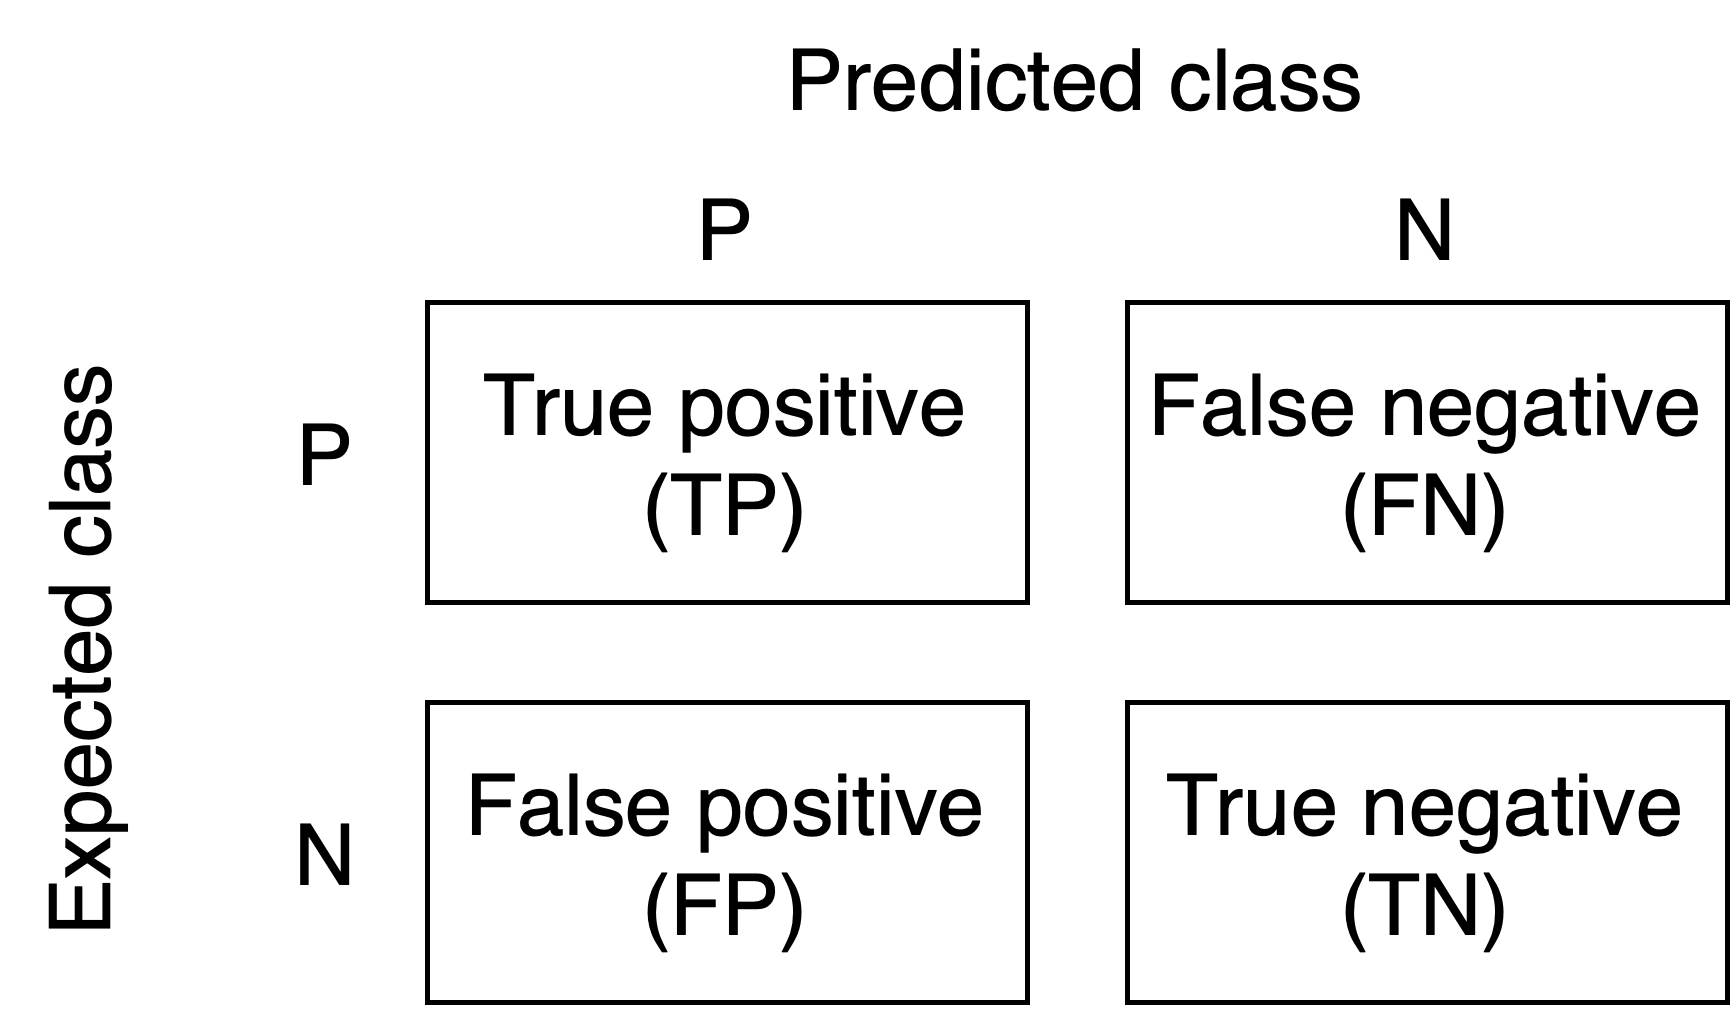
\includegraphics[width=0.4\textwidth]{author/part3/figures/conf_matrix.png}
					\caption{Матрица ошибок}
					\label{fig:conf_matrix}
				\end{figure}
				
				ROC-кривая -- это график, в котором, основываясь на заданном пороге решения классификатора, рассчитываются доли ложноположительных и истинно положительных исходов. Основываясь на ROC-кривой, высчитывается AUC-показатель (площадь под кривой), которая используется в качестве характеристики качества модели.
				
				В интеллектуальной среде проектирования данный этап соответствует выполнению \textit{действия оценки эффективности и.н.с.}.
				
				Рассмотрим пример выполнения описанных этапов разработчиком для конкретной задачи -- \textit{классификации цифр из выборки рукописных цифр MNIST}:
				
				\textbf{1.} Исходными данными задачи является: выборка из 70.000 изображений, предварительно разделенная на обучающую (60.000 изображений) и контрольную (10.000 изображений) выборки. Каждое изображение представлено двумерным массивом 28Х28 чисел из интервала [0, 255], числа представляют определенный оттенок серого цвета. Помимо этого каждому изображению соответствует метка класса, соответствующая конкретной цифре от 0 до 9.
				
				Ставится задача: \textit{обучить модель, которая будет принимать на вход двумерный массив данных и возвращать метку класса, соответствующей распознанной цифре.}
				
				Таким образом, тип решаемой задачи -- \textbf{классификационная}, природа данных задачи -- \textbf{изображения}.
				
				\textbf{2.} В рассматриваемой выборке отсутствуют аномалии, ошибочные данные, признаки с отсутствующими значениями.
				
				\textbf{3.} В рассматриваемой задаче отсутствуют несодержательные признаки.
				
				\textbf{4.} В качестве метода предобработки данных используем масштабирование признаков, а именно нормализацию на отрезок [0, 1].
				
				\textbf{5.} Выполним разбиение обучающей части данных на обучающую и валидационную выборки в соотношении 4:1 (48.000 в обучающей и 12.000 в валидационной).
				
				\textbf{6.} Так как выборка включает в себя изображения, будем использовать сверточную нейронную сеть.
				
				\textbf{7.} Не требуется.
				
				\textbf{8.} В качестве оптимизационного алгоритма будем использовать метод стохастического градиентного спуска (SGD).
				
				\textbf{9.} Так как решается задача классификации, выберем в качестве минимизируемой функции кросс-энтропийную функцию потерь.
				
				\textbf{10.} В качестве начальной инициализации будем использовать инициализацию по методу Кайминга.
				
				\textbf{11.} На этапе 6 и 8 было определено, что для решения задачи будет использоваться сверточная нейронная сеть. При использовании one-hot кодирования в последнем полносвязном слое будет 10 нейронов по числу классов в задаче.
				
				Для упрощения будем использовать архитектуру, изображенную на рис. \ref{fig:model}, не содержащую промежуточные слои.
				
				\begin{figure}[h]
					\centering
					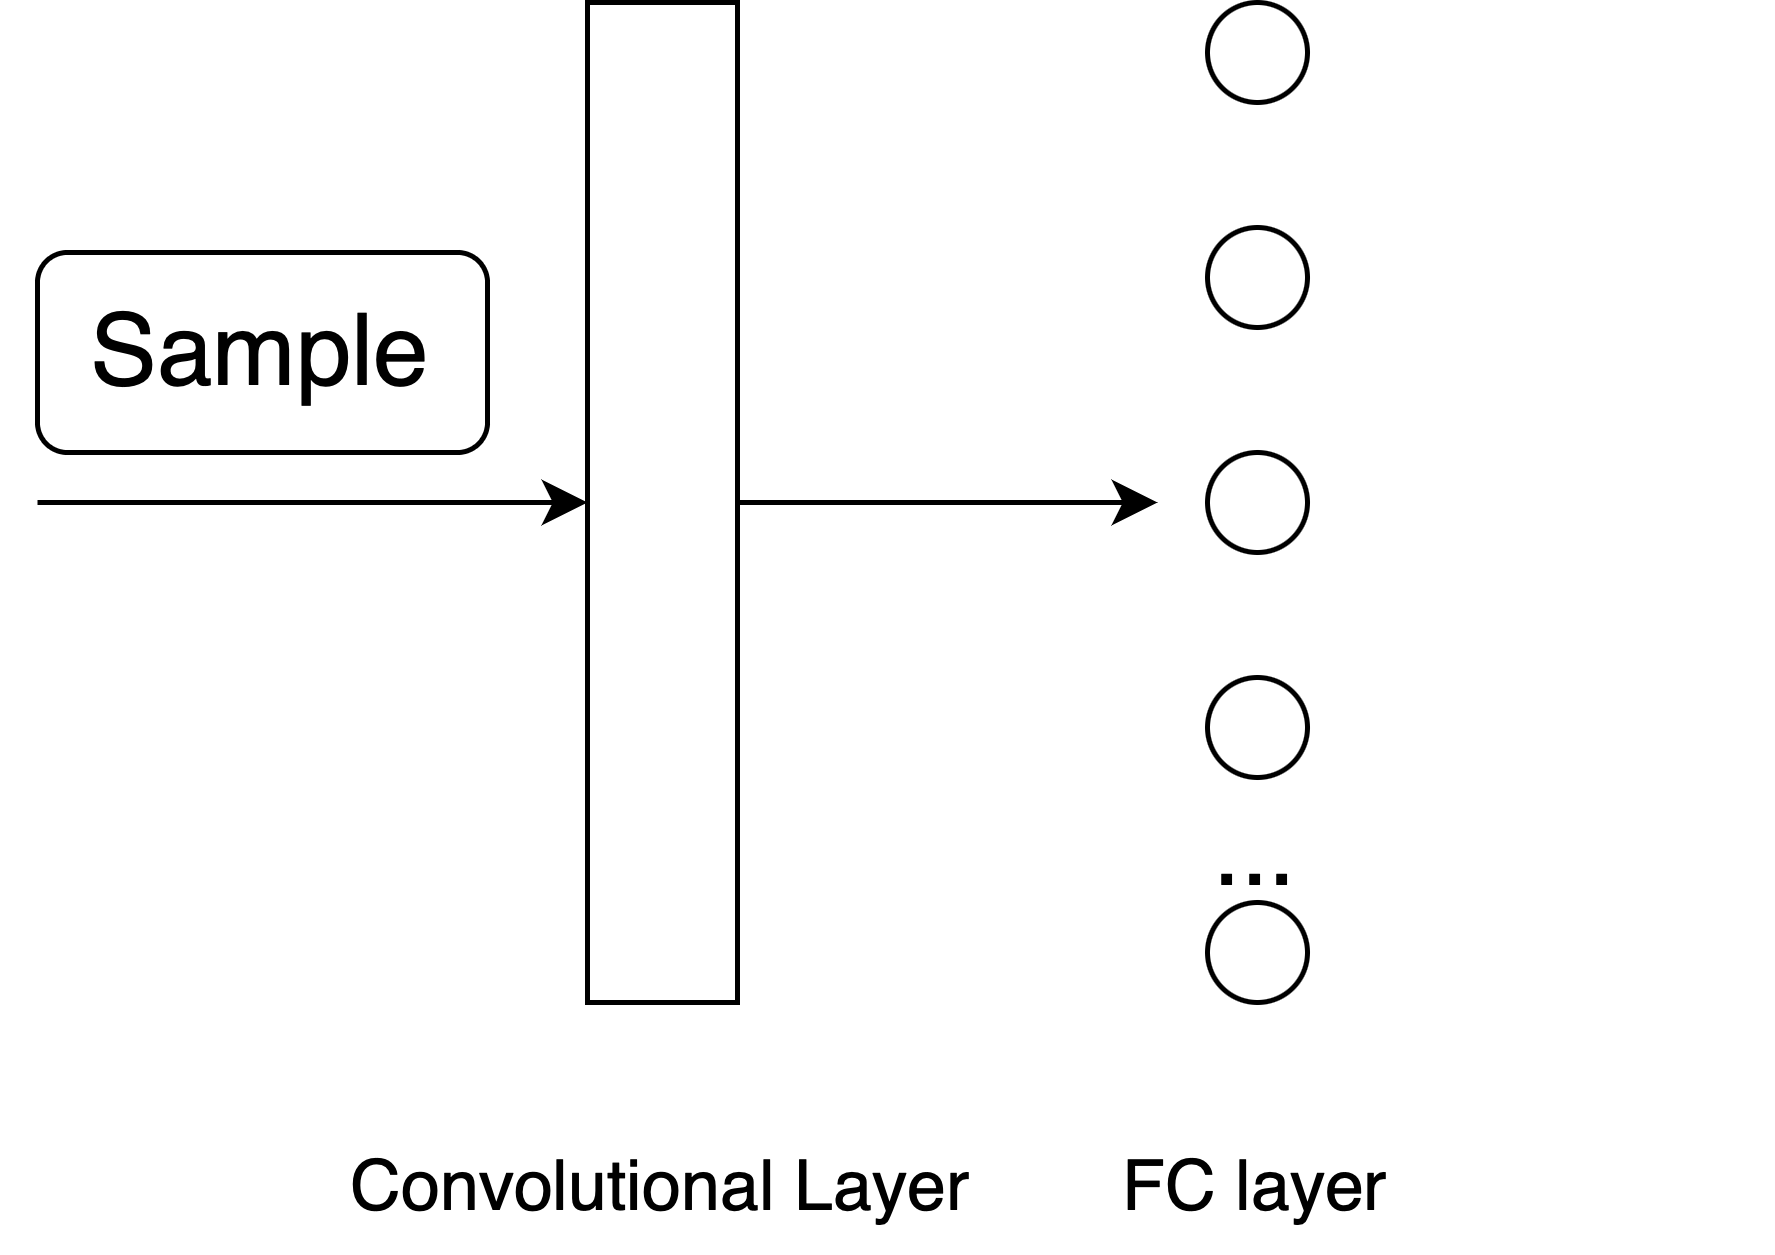
\includegraphics[width=0.4\textwidth]{author/part3/figures/model.png}
					\caption{Архитектура и.н.с., решающая задачу классификации цифр}
					\label{fig:model}
				\end{figure}
				
				Для нахождения оптимального набора гиперпараметров будем применять метод случайного поиска.
				
				Перечислим кортежи, из которых будут сэмплироваться гиперпараметры:
				\begin{itemize}
					\item Скорость обучения -- (0.9, 0.1, 0.01, 0.001)
					\item Количество нейронов в сверточном слое -- (5, 10, 15, 20)
					\item Размер ядра свертки -- (3, 5, 7, 9)
					\item Моментный параметр -- (0, 0.5, 0.9)
					\item Размер мини-батча -- (16, 32, 64, 128)
				\end{itemize}
				
				После определения данных параметров и оценки эффективности работы алгоритма, получим следующую таблицу:
				
				\begin{table}[ht]
					\caption{Результаты решения задачи \\(используемые сокращения: mbs -- mini-batch size, ks -- kernel size, lr -- learning rate, cnc -- convolutional neurons count, acc -- accuracy, it -- iterations count)}
					\centering
					\begin{tabular}{c c c c c c c c}
						\hline\hline
						\# & mbs & ks & lr & momentum & cnc & acc & it \\ [0.5ex] % inserts table %heading
						\hline
						1&128&3&0.001&0.5&10&0.9033&10 \\
						2&64&9&0.9&0&15&0.1039&1 \\
						3&32&3&0.01&0.5&20&0.9741&10\\
						4&32&7&0.01&0.5&15&0.9794&10\\
						5&16&9&0.001&0.5&20&0.9189&2\\
						6&64&3&0.1&0.5&10&0.9736&10\\
						7&64&7&0.001&0.9&15&0.9007&1\\
						8&32&9&0.1&0.5&5&0.9806&10\\
						9&128&5&0.1&0.5&20&0.98&10\\
						10&32&9&0.01&0.9&5&0.9806&10\\
						11&128&3&0.001&0.9&10&0.893&1\\
						12&32&5&0.9&0.9&20&0.1008&1\\
						13&16&9&0.9&0.5&20&0.0976&1\\
						14&32&7&0.9&0.9&15&0.0932&1\\
						15&128&5&0.01&0.5&20&0.9197&2\\
						16&16&3&0.001&0.5&10&0.904&1\\
						17&16&9&0.001&0&20&0.8866&1\\
						18&128&9&0.1&0.5&5&0.9793&10\\
						19&128&3&0.001&0&10&0.6697&1\\
						20&16&3&0.1&0&15&0.9729&4\\
						21&32&7&0.9&0.5&15&0.1048&1\\
						22&128&7&0.9&0&15&0.1113&1\\
						23&64&9&0.01&0.5&10&0.9482&2\\
						24&16&7&0.9&0&20&0.0985&1\\
						25&16&3&0.1&0.5&5&0.9558&2\\
						26&64&7&0.01&0.9&15&0.9839&10\\
						27&16&7&0.1&0&10&0.9836&10\\
						28&16&5&0.01&0&20&0.9608&2\\
						29&16&5&0.01&0.9&20&0.9847&10\\
						30&32&5&0.01&0.5&15&0.9532&2\\
						\hline
					\end{tabular}
					\label{table:nonlin}
				\end{table}
				
				Можно заметить, что лучший результат (acc = 0.9839) по обобщающей способности на валидационной выборке был получен при следующих параметрах: mbs = 64, ks = 7, lr = 0.01, momentum = 0.9, cnc = 15.
				
				\textbf{12.} В качестве критерия останова нами был выбран самый простой критерий по достижению заданного количества эпох обучения. Дообучение не проводилось, для оценки обобщающей способности использовалась модель, полученная после выполнения процедуры подбора гиперпараметров. Обобщающая способность на тестовой выборке составила \textbf{0.9853}, т.е. \textbf{98.53\%}.
				
				\textbf{13.} Построив матрицу ошибок на основании обученной модели и тестовой выборки, получим результат, проиллюстрированный на рис. \ref{fig:conf_matrix_result}
				
				\begin{figure}[h]
					\centering
					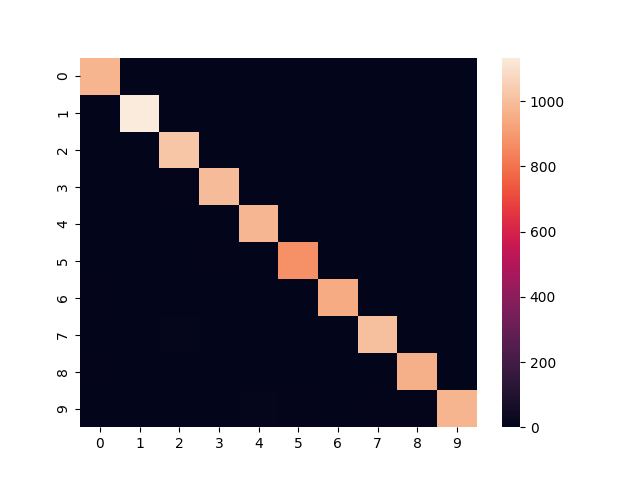
\includegraphics[width=0.55\textwidth]{author/part3/figures/conf_matrix_result.png}
					\caption{Матрица ошибок для задачи MNIST}
					\label{fig:conf_matrix_result}
				\end{figure}
				
				Мы получили матрицу с явно выраженным диагональным преобладанием, таким образом полученная модель делает относительно небольшое число ошибок.
				
				Исходя из анализа этапов построения и.н.с., которые выполняют разработчики, можно вывести следующую классификацию действий по построению и.н.с.:

				\begin{SCn}
					\scnheader{действие по построению и.н.с.}
					\begin{scnrelfromset}{декомпозиция}
						\scnitem{действие по обработке выборки}
						\begin{scnrelfromset}{декомпозиция}
							\scnitem{действие поиска подходящей обучающей выборки}
							\scnitem{действие формирования требований к обучающей выборке}
							\scnitem{действие очистки выборки}
							\scnitem{действие выявления содержательных признаков}
							\scnitem{действие трансформации выборки}
							\scnitem{действие разбиения выборки}
						\end{scnrelfromset}
						
						\scnitem{действие по проектированию и.н.с.}
						\begin{scnrelfromset}{декомпозиция}
							\scnitem{действие выбора класса нейросетевых методов}
							\scnitem{действие формирования спецификации входов и выходов и.н.с.}
						\end{scnrelfromset}
						
						\scnitem{действие обучения и.н.с.}
						\begin{scnrelfromset}{декомпозиция}
							\scnitem{действие выбора метода оптимизации}
							\scnitem{действие выбора минимизируемой функции ошибки}
							\scnitem{действие начальной инициализации и.н.с.}
							\scnitem{действие выбора гиперпараметров и.н.с.}
							\scnitem{действие обучения и.н.с.}
							\scnitem{действие оценки эффективности и.н.с.}
						\end{scnrelfromset}
					\end{scnrelfromset}
				\end{SCn}
				
				Реализация интерпретатора описанных в данной главе действий по построению и.н.с. и описания в базе знаний экспертных знаний разработчиков и.н.с. (а значит реализация интеллектуальной среды проектирования и.н.с.) позволит автоматически, исходя из описания задачи, генерировать нейросетевые методы в памяти ostis-системы, что является одним из ключевых направлений развития данной работы.

%%%%%%%%%%%%%%%%%%%%%%%%% referenc.tex %%%%%%%%%%%%%%%%%%%%%%%%%%%%%%
% sample references
% %
% Use this file as a template for your own input.
%
%%%%%%%%%%%%%%%%%%%%%%%% Springer-Verlag %%%%%%%%%%%%%%%%%%%%%%%%%%
%
% BibTeX users please use
% \bibliographystyle{}
% \bibliography{}
%
\biblstarthook{In view of the parallel print and (chapter-wise) online publication of your book at \url{www.springerlink.com} it has been decided that -- as a genreral rule --  references should be sorted chapter-wise and placed at the end of the individual chapters. However, upon agreement with your contact at Springer you may list your references in a single seperate chapter at the end of your book. Deactivate the class option \texttt{sectrefs} and the \texttt{thebibliography} environment will be put out as a chapter of its own.\\\indent
References may be \textit{cited} in the text either by number (preferred) or by author/year.\footnote{Make sure that all references from the list are cited in the text. Those not cited should be moved to a separate \textit{Further Reading} section or chapter.} If the citatiion in the text is numbered, the reference list should be arranged in ascending order. If the citation in the text is author/year, the reference list should be \textit{sorted} alphabetically and if there are several works by the same author, the following order should be used:
\begin{enumerate}
\item all works by the author alone, ordered chronologically by year of publication
\item all works by the author with a coauthor, ordered alphabetically by coauthor
\item all works by the author with several coauthors, ordered chronologically by year of publication.
\end{enumerate}
The \textit{styling} of references\footnote{Always use the standard abbreviation of a journal's name according to the ISSN \textit{List of Title Word Abbreviations}, see \url{http://www.issn.org/en/node/344}} depends on the subject of your book:
\begin{itemize}
\item The \textit{two} recommended styles for references in books on \textit{mathematical, physical, statistical and computer sciences} are depicted in ~\cite{science-contrib, science-online, science-mono, science-journal, science-DOI} and ~\cite{phys-online, phys-mono, phys-journal, phys-DOI, phys-contrib}.
\item Examples of the most commonly used reference style in books on \textit{Psychology, Social Sciences} are~\cite{psysoc-mono, psysoc-online,psysoc-journal, psysoc-contrib, psysoc-DOI}.
\item Examples for references in books on \textit{Humanities, Linguistics, Philosophy} are~\cite{humlinphil-journal, humlinphil-contrib, humlinphil-mono, humlinphil-online, humlinphil-DOI}.
\item Examples of the basic Springer style used in publications on a wide range of subjects such as \textit{Computer Science, Economics, Engineering, Geosciences, Life Sciences, Medicine, Biomedicine} are ~\cite{basic-contrib, basic-online, basic-journal, basic-DOI, basic-mono}. 
\end{itemize}
}

\begin{thebibliography}{99.}%
% and use \bibitem to create references.
%
% Use the following syntax and markup for your references if 
% the subject of your book is from the field 
% "Mathematics, Physics, Statistics, Computer Science"
%
% Contribution 
\bibitem{science-contrib} Broy, M.: Software engineering --- from auxiliary to key technologies. In: Broy, M., Dener, E. (eds.) Software Pioneers, pp. 10-13. Springer, Heidelberg (2002)
%
% Online Document
\bibitem{science-online} Dod, J.: Effective substances. In: The Dictionary of Substances and Their Effects. Royal Society of Chemistry (1999) Available via DIALOG. \\
\url{http://www.rsc.org/dose/title of subordinate document. Cited 15 Jan 1999}
%
% Monograph
\bibitem{science-mono} Geddes, K.O., Czapor, S.R., Labahn, G.: Algorithms for Computer Algebra. Kluwer, Boston (1992) 
%
% Journal article
\bibitem{science-journal} Hamburger, C.: Quasimonotonicity, regularity and duality for nonlinear systems of partial differential equations. Ann. Mat. Pura. Appl. \textbf{169}, 321--354 (1995)
%
% Journal article by DOI
\bibitem{science-DOI} Slifka, M.K., Whitton, J.L.: Clinical implications of dysregulated cytokine production. J. Mol. Med. (2000) doi: 10.1007/s001090000086 
%
\bigskip

% Use the following (APS) syntax and markup for your references if 
% the subject of your book is from the field 
% "Mathematics, Physics, Statistics, Computer Science"
%
% Online Document
\bibitem{phys-online} J. Dod, in \textit{The Dictionary of Substances and Their Effects}, Royal Society of Chemistry. (Available via DIALOG, 1999), 
\url{http://www.rsc.org/dose/title of subordinate document. Cited 15 Jan 1999}
%
% Monograph
\bibitem{phys-mono} H. Ibach, H. L\"uth, \textit{Solid-State Physics}, 2nd edn. (Springer, New York, 1996), pp. 45-56 
%
% Journal article
\bibitem{phys-journal} S. Preuss, A. Demchuk Jr., M. Stuke, Appl. Phys. A \textbf{61}
%
% Journal article by DOI
\bibitem{phys-DOI} M.K. Slifka, J.L. Whitton, J. Mol. Med., doi: 10.1007/s001090000086
%
% Contribution 
\bibitem{phys-contrib} S.E. Smith, in \textit{Neuromuscular Junction}, ed. by E. Zaimis. Handbook of Experimental Pharmacology, vol 42 (Springer, Heidelberg, 1976), p. 593
%
\bigskip
%
% Use the following syntax and markup for your references if 
% the subject of your book is from the field 
% "Psychology, Social Sciences"
%
%
% Monograph
\bibitem{psysoc-mono} Calfee, R.~C., \& Valencia, R.~R. (1991). \textit{APA guide to preparing manuscripts for journal publication.} Washington, DC: American Psychological Association.
%
% Online Document
\bibitem{psysoc-online} Dod, J. (1999). Effective substances. In: The dictionary of substances and their effects. Royal Society of Chemistry. Available via DIALOG. \\
\url{http://www.rsc.org/dose/Effective substances.} Cited 15 Jan 1999.
%
% Journal article
\bibitem{psysoc-journal} Harris, M., Karper, E., Stacks, G., Hoffman, D., DeNiro, R., Cruz, P., et al. (2001). Writing labs and the Hollywood connection. \textit{J Film} Writing, 44(3), 213--245.
%
% Contribution 
\bibitem{psysoc-contrib} O'Neil, J.~M., \& Egan, J. (1992). Men's and women's gender role journeys: Metaphor for healing, transition, and transformation. In B.~R. Wainrig (Ed.), \textit{Gender issues across the life cycle} (pp. 107--123). New York: Springer.
%
% Journal article by DOI
\bibitem{psysoc-DOI}Kreger, M., Brindis, C.D., Manuel, D.M., Sassoubre, L. (2007). Lessons learned in systems change initiatives: benchmarks and indicators. \textit{American Journal of Community Psychology}, doi: 10.1007/s10464-007-9108-14.
%
%
% Use the following syntax and markup for your references if 
% the subject of your book is from the field 
% "Humanities, Linguistics, Philosophy"
%
\bigskip
%
% Journal article
\bibitem{humlinphil-journal} Alber John, Daniel C. O'Connell, and Sabine Kowal. 2002. Personal perspective in TV interviews. \textit{Pragmatics} 12:257--271
%
% Contribution 
\bibitem{humlinphil-contrib} Cameron, Deborah. 1997. Theoretical debates in feminist linguistics: Questions of sex and gender. In \textit{Gender and discourse}, ed. Ruth Wodak, 99--119. London: Sage Publications.
%
% Monograph
\bibitem{humlinphil-mono} Cameron, Deborah. 1985. \textit{Feminism and linguistic theory.} New York: St. Martin's Press.
%
% Online Document
\bibitem{humlinphil-online} Dod, Jake. 1999. Effective substances. In: The dictionary of substances and their effects. Royal Society of Chemistry. Available via DIALOG. \\
http://www.rsc.org/dose/title of subordinate document. Cited 15 Jan 1999
%
% Journal article by DOI
\bibitem{humlinphil-DOI} Suleiman, Camelia, Daniel C. O'Connell, and Sabine Kowal. 2002. `If you and I, if we, in this later day, lose that sacred fire...': Perspective in political interviews. \textit{Journal of Psycholinguistic Research}. doi: 10.1023/A:1015592129296.
%
%
%
\bigskip
%
%
% Use the following syntax and markup for your references if 
% the subject of your book is from the field 
% "Computer Science, Economics, Engineering, Geosciences, Life Sciences"
%
%
% Contribution 
\bibitem{basic-contrib} Brown B, Aaron M (2001) The politics of nature. In: Smith J (ed) The rise of modern genomics, 3rd edn. Wiley, New York 
%
% Online Document
\bibitem{basic-online} Dod J (1999) Effective Substances. In: The dictionary of substances and their effects. Royal Society of Chemistry. Available via DIALOG. \\
\url{http://www.rsc.org/dose/title of subordinate document. Cited 15 Jan 1999}
%
% Journal article by DOI
\bibitem{basic-DOI} Slifka MK, Whitton JL (2000) Clinical implications of dysregulated cytokine production. J Mol Med, doi: 10.1007/s001090000086
%
% Journal article
\bibitem{basic-journal} Smith J, Jones M Jr, Houghton L et al (1999) Future of health insurance. N Engl J Med 965:325--329
%
% Monograph
\bibitem{basic-mono} South J, Blass B (2001) The future of modern genomics. Blackwell, London 
%
\end{thebibliography}
